\PassOptionsToPackage{table}{xcolor}
%\documentclass{beamer}
\documentclass[compress]{beamer}
%\usetheme{Epam}
\usetheme{Copenhagen}
\usepackage{xcolor}
\usepackage{listings}
\usepackage{graphicx}
\usepackage[utf8]{inputenc}
\usepackage{datetime}
\usepackage{beamerthemesplit}
%\beamertemplatenavigationsymbolsempty
\usepackage{listingsutf8}
\usepackage{ragged2e}
\usepackage{hyperref}
\lstset{ %
  language=C,                      % the language of the code
%  basicstyle=\ttfamily,           % the size of the fonts that are used for the code
%  basicstyle=\ttfamily\tiny,      % the size of the fonts that are used for the code
  basicstyle=\ttfamily\scriptsize, % the size of the fonts that are used for the code
  numbers=left,                    % where to put the line-numbers
  numberstyle=\tiny\color{gray},   % the style that is used for the line-numbers
  stepnumber=1,                    % the step between two line-numbers. If it's 1, each line 
                                   % will be numbered
  numbersep=5pt,                   % how far the line-numbers are from the code
  %backgroundcolor=\color{gray},   % choose the background color. You must add \usepackage{color}
  showspaces=false,               % show spaces adding particular underscores
  showstringspaces=false,         % underline spaces within strings
  showtabs=false,                 % show tabs within strings adding particular underscores
%  frame=shadowbox,                   % adds a frame around the code
  rulecolor=\color{black},        % if not set, the frame-color may be changed on line-breaks within not-black text (e.g. commens (green here))
  tabsize=4,                      % sets default tabsize to 4 spaces
  captionpos=,                   % sets the caption-position to bottom
  breaklines=false,                % sets automatic line breaking
  breakatwhitespace=false,        % sets if automatic breaks should only happen at whitespace
  title=\lstname,                 % show the filename of files included with \lstinputlisting;
                                  % also try caption instead of title
  keywordstyle=\color{blue},      % keyword style
  commentstyle=\color{mygreen},   % comment style
  stringstyle=\color{magenta},    % string literal style
%  escapeinside={\%*}{*)},        % if you want to add a comment within your code
  inputencoding=utf8,
  extendedchars=\true,
  morekeywords={*,..., restrict, alignof, alignas, bool, true, false, size_t, ssize_t, inline, \_Noreturn, noreturn},
  breakautoindent=false,
  breakindent=1pt,
}

%\setbeameroption{show only notes}
%\usepackage{pgfpages}
%\setbeameroption{show notes}
%\setbeameroption{show notes on second screen=right}

\setbeamertemplate{navigation symbols}{}

\definecolor{oddrow}{RGB}{100,149,237}
\definecolor{evenrow}{RGB}{135,206,250}
\def\mybs{\textbackslash}
\newcommand{\qq}{\symbol{34}} % the decimal ascii code for "
\newcommand{\sq}{\symbol{39}} % the decimal ascii code for '

\makeatletter
\newcommand{\rmnum}[1]{\romannumeral #1}
\newcommand{\Rmnum}[1]{\expandafter\@slowromancap\romannumeral #1@}
\newcommand{\inc}{\symbol{45}\symbol{45}}
\newcommand{\dec}{\symbol{43}\symbol{43}}
\newcommand{\lsh}{\symbol{60}\symbol{60}}
\newcommand{\rsh}{\symbol{62}\symbol{62}}
\makeatother

\newcommand{\specialcell}[2][c]{%
  \begin{tabular}[#1]{@{}c@{}}#2\end{tabular}}
\newcommand{\specialcellhl}[2][l]{%
  \begin{tabular}[#1]{@{}l@{}}#2\end{tabular}}
\newcommand{\specialcellhc}[2][c]{%
  \begin{tabular}[#1]{@{}c@{}}#2\end{tabular}}

\definecolor{mygreen}{rgb}{0,0.6,0}
\definecolor{olive}{rgb}{0.3, 0.4, .1}
\definecolor{fore}{RGB}{249,242,215}
\definecolor{back}{RGB}{51,51,51}
\definecolor{title}{RGB}{255,0,90}
\definecolor{dgreen}{rgb}{0.,0.6,0.}
\definecolor{gold}{rgb}{1.,0.84,0.}
\definecolor{JungleGreen}{cmyk}{0.99,0,0.52,0}
\definecolor{BlueGreen}{cmyk}{0.85,0,0.33,0}
\definecolor{RawSienna}{cmyk}{0,0.72,1,0.45}
\definecolor{Magenta}{cmyk}{0,1,0,0}

\newcommand{\kwblue}[1]{\texttt{\textcolor{blue}{#1}}}
\newcommand{\kwblack}[1]{\texttt{\textcolor{black}{#1}}}
\newcommand{\kwred}[1]{\texttt{\textcolor{red}{#1}}}
\newcommand{\kwmagenta}[1]{\texttt{\textcolor{Magenta}{#1}}}

%\newcommand{\hdr}[1]{\textless{#1}\textgreater{}}
\newcommand{\hdr}[1]{\textless{\kwmagenta{#1}}\textgreater{}}

\author[\href{mailto:vasili_slapik@epam.com}{Vasili Slapik}]{\texorpdfstring{Vasili Slapik\newline\href{mailto:vasili_slapik@epam.com}{vasili\_slapik@epam.com}}{Vasili Slapik}}


\title{\Rmnum{3}. Operations and expressions}

\begin{document}

% TODO:
% explain that every expression has calculated value even x=5 , 5; main; which can be assigned to another expression
% https://www.securecoding.cert.org/confluence/pages/viewpage.action?pageId=6422581 (INT10-C. Do not assume a positive remainder when using the % operator)

%%%%%%%%%%%%%%%%%%%%%%%%%%%%%%%%%%%%%%%%%%%%%%%%%%%%%%%%%%%%%%%%%%%%%%%%%%%%%%%%%
\frame{\titlepage}
%%%%%%%%%%%%%%%%%%%%%%%%%%%%%%%%%%%%%%%%%%%%%%%%%%%%%%%%%%%%%%%%%%%%%%%%%%%%%%%%%
\begin{frame}{Operators}
    \only<1>{
        \begin{tabular}{lllll}
            \specialcell{\textbf{arithmetic}     \\
                \texttt{a + b}                   \\
                \texttt{a - b}                   \\
                \texttt{a * b}                   \\
                \texttt{a / b}                   \\
                \texttt{a \% b}                  \\
                \texttt{+a}                      \\
                \texttt{-a}                      \\
            } &
            \specialcell{\textbf{assignment}     \\
                \texttt{a = b}                   \\
                \texttt{a += b}                  \\
                \texttt{a -= b}                  \\
                \texttt{a *= b}                  \\
                \texttt{a /= b}                  \\
                \note{not for double and float}
                \texttt{a \%= b}                 \\
                \texttt{a \&= b}                 \\
                \texttt{a |= b}                  \\
                \texttt{a \textasciicircum{=} b} \\
                \texttt{a \lsh= b}               \\
                \texttt{a \rsh= b}               \\
            } &
            \specialcell{\textbf{bitwise}        \\
                \texttt{\textasciitilde{a}}      \\
                \texttt{a \& b}                  \\
                \texttt{a | b}                   \\
                \texttt{a \textasciicircum{ b}}  \\
                \texttt{a \lsh{} b}              \\
                \texttt{a \rsh{} b}              \\
            } &
            \specialcell{\textbf{comparison}    \\
                \texttt{a == b}                  \\
                \texttt{a != b}                  \\
                \texttt{a < b}                   \\
                \texttt{a > b}                   \\
                \texttt{a <= b}                  \\
                \texttt{a >= b}                  \\
            } &
            \specialcell{\textbf{logical}        \\
                \texttt{!a}                      \\
                \texttt{a \&\& b}                \\
                \texttt{a || b}                  \\
            } \\
        \end{tabular}
    }
    \only<2>{
        \begin{tabular}{llll}
            \specialcell{\textbf{increment} \\ \textbf{decrement}  \\
                \texttt{a\inc}                   \\
                \texttt{a\dec}                   \\
                \texttt{\inc{}a}                 \\
                \texttt{\dec{}a}                 \\
            } &
            \specialcell{\textbf{member access}  \\
                \texttt{s.b}                     \\
                \texttt{s->b}                    \\
            } &
            \specialcell{\textbf{reference} \\ \textbf{dereference}  \\
                \texttt{\&a}                     \\
                \texttt{*a}                      \\
                \texttt{a[b]}                    \\
            } &
            \specialcell{\textbf{other}          \\
                \texttt{func(...)}               \\
                \texttt{a, b}                    \\
                \texttt{(type)a}                 \\
                \texttt{a ? b : c}               \\
                \texttt{sizeof(a)}               \\
                \texttt{\_Alignof(a)} (C11)      \\
            } \\
        \end{tabular}
    }
\end{frame}
%%%%%%%%%%%%%%%%%%%%%%%%%%%%%%%%%%%%%%%%%%%%%%%%%%%%%%%%%%%%%%%%%%%%%%%%%%%%%%%%%
\begin{frame}{sizeof operator}
    \lstinputlisting{03_sizeof.c}
\end{frame}
%%%%%%%%%%%%%%%%%%%%%%%%%%%%%%%%%%%%%%%%%%%%%%%%%%%%%%%%%%%%%%%%%%%%%%%%%%%%%%%%%
\begin{frame}{Operators precedence}
    \only<1>{
        \justifying
        Precedence and associativity don't tell you about order of evaluation. They only tell you about grouping of operands.
    }
    \only<2>{
        \lstinputlisting{03_associativity.c}
    }
    \only<3>{
        \lstinputlisting{03_associativity_2.c}
    }
    \only<4>{
        \rowcolors{1}{oddrow}{evenrow}
        \begin{tabular}{l|c|l|l}
            \textbf{P} & \textbf{Operator} & \textbf{Description} & \textbf{Associativity} \\
            1 &
            \specialcell{
                \texttt{( )}                        \\
                \texttt{[ ]}                        \\
                \texttt{.}                          \\
                \texttt{->}                         \\
                \texttt{a\inc{} a\dec{}}            \\
            } &
            \specialcellhl{
                Function call or sub-expression     \\
                Array subscript                     \\
                Member selection via object name    \\
                Member selection via pointer        \\
                Postfix increment/decrement         \\
            } & left-to-right                       \\
            2 &
            \specialcell{
                \texttt{\inc{}a \dec{}a}            \\
                \texttt{+  -}                       \\
                \texttt{! \textasciitilde}          \\
                \texttt{(type)}                     \\
                \texttt{*}                          \\
                \texttt{\&}                         \\
                \texttt{sizeof}                     \\
            } &
            \specialcellhl{
                Prefix increment/decrement          \\
                Unary plus/minus                    \\
                Logical negation/bitwise complement \\
                Cast to type                        \\
                Dereference                         \\
                Address (of operand)                \\
                Determine size in bytes             \\
            } & right-to-left                       \\
            3 &
            \texttt{* / \%} &
            Multiplication/division/modulus &
            left-to-right                           \\
        \end{tabular}
    }

    \only<5>{
        \rowcolors{1}{oddrow}{evenrow}
        \begin{tabular}{l|c|l|l}
            \textbf{P} & \textbf{Operator} & \textbf{Description} & \textbf{Associativity} \\

            4 & \texttt{+ -}    & Addition/subtraction                     & left-to-right  \\
            5 & \texttt{<< >>}  & Bitwise shift (left / right)             & left-to-right  \\

            6 &
            \specialcell{
                \texttt{< <=} \\
                \texttt{> >=} \\
            } &
            \specialcellhl{
                Less than / less than or equal      \\
                Greater than/ greater than or equal \\
            } &
            left-to-right \\

            7  & \texttt{== !=} & Is equal / is not equal & left-to-right \\
            8  & \texttt{\&}    & Bitwise AND             & left-to-right \\
            9  & \texttt{\^}    & Bitwise exclusive OR    & left-to-right \\
            10 & \texttt{|}     & Bitwise inclusive OR    & left-to-right \\
            11 & \texttt{\&\&}  & Logical AND             & left-to-right \\
            12 & \texttt{||}    & Logical OR              & left-to-right \\
            13 & \texttt{?:}    & Ternary conditional     & right-to-left \\
        \end{tabular}
    }

    \only<6>{
        \rowcolors{1}{oddrow}{evenrow}
        \begin{tabular}{l|c|l|l}
            \textbf{P} & \textbf{Operator} & \textbf{Description} & \textbf{Associativity} \\
            14 &
            \specialcell{
                \texttt{=}           \\
                \texttt{+=}          \\
                \texttt{-=}          \\
                \texttt{*=}          \\
                \texttt{/=}          \\
                \texttt{\%=}         \\
                \texttt{\&=}         \\
                \texttt{\^{}=}       \\
                \texttt{|=}          \\
                \texttt{<<=}         \\
                \texttt{>>=}         \\
            } &
            \specialcell{
                Assignment                                \\
                Addition assignment                       \\
                Subtraction assignment                    \\
                Multiplication assignment                 \\
                Division assignment                       \\
                Modulus assignment                        \\
                Bitwise AND assignment                    \\
                Bitwise exclusive OR assignment           \\
                Bitwise inclusive OR assignment           \\
                Bitwise shift left assignment             \\
                Bitwise shift right assignment            \\
            } & right-to-left \\

            15 & , & Comma (separate expressions) & left-to-right \\

        \end{tabular}
    }
\end{frame}

%%%%%%%%%%%%%%%%%%%%%%%%%%%%%%%%%%%%%%%%%%%%%%%%%%%%%%%%%%%%%%%%%%%%%%%%%%%%%%%
\begin{frame}{Precedence problems of C operators}
    \rowcolors{1}{oddrow}{evenrow}
    \scriptsize{
    \begin{center}
        \begin{tabular}{c|c|c|c}
            \specialcellhc{\textbf{Precedence}  \\ \textbf{problem}}      &
            \specialcellhc{\textbf{Expression}}                           &
            \specialcellhc{\textbf{What people} \\ \textbf{expect}}       &
            \specialcellhc{\textbf{What They}   \\ \textbf{Actually Get}}
            \\
            \specialcellhc{\texttt{.} is higher\\than \texttt{*}}         &
            \texttt{*p.f}                                                 &
            \texttt{(*p).f}                                               &
            \texttt{*(p.f)}
            \\
            \specialcellhc{\texttt{[]} is higher\\than \texttt{*}}                                       &
            \texttt{int *ap[]}                                                                           &
            \specialcellhc{\texttt{ap} is a pointer\\to array of \texttt{int}s:\\ \texttt{int (*ap)[]}}  &
            \specialcellhc{\texttt{ap} is an array\\of pointers to \texttt{int}:\\ \texttt{int *(ap[])}}
            \\
            \specialcellhc{function \texttt{()} is\\higher than \texttt{*}}                                       &
            \texttt{int *fp()}                                                                                    &
            \specialcellhc{\texttt{fp} is a pointer\\to function\\returning \texttt{int}:\\ \texttt{int (*fp)()}} &
            \specialcellhc{\texttt{fp} is a function\\returning\\pointer to \texttt{int}:\\ \texttt{int *(fp())}}
            \\
            \specialcellhc{\texttt{==} and \texttt{!=} higher\\than bitwise\\operators} &
            \specialcellhc{\texttt{val \& mask != 0}}                                   &
            \specialcellhc{\texttt{(val \& mask) != 0}}                                 &
            \specialcellhc{\texttt{val \& (mask != 0)}}
            \\
            \specialcellhc{\texttt{==} and \texttt{!=} higher\\than assignment}         &
            \specialcellhc{\texttt{c = f() != 0}}                                       &
            \specialcellhc{\texttt{(c = f()) != 0}}                                     &
            \specialcellhc{\texttt{c = (f() != 0)}}
            \\
            \specialcellhc{arithmetic higher\\than shift}                               &
            \specialcellhc{\texttt{msb \lsh{} 4 + lsb}}                                 &
            \specialcellhc{\texttt{(msb \lsh{} 4) + lsb}}                               &
            \specialcellhc{\texttt{msb \lsh{} (4 + lsb)}}
            \\
            \specialcellhc{\texttt{,} has lowest\\precedence of\\all operators}         &
            \specialcellhc{\texttt{i = 1,2}}                                            &
            \specialcellhc{\texttt{i = (1,2)}}                                          &
            \specialcellhc{\texttt{(i = 1), 2}}
            \\

        \end{tabular}
    \end{center}
    }
\end{frame}
%%%%%%%%%%%%%%%%%%%%%%%%%%%%%%%%%%%%%%%%%%%%%%%%%%%%%%%%%%%%%%%%%%%%%%%%%%%%%%%
\begin{frame}{Common traps}
    \only<1>{
        \lstinputlisting{03_trap1.c}
    }
    \only<2>{
        \lstinputlisting{03_trap2.c}
    }
    \only<3>{
        \lstinputlisting{03_trap3.c}
    }
    \only<4>{
        \lstinputlisting{03_trap4.c}
    }
    \only<5>{
        \lstinputlisting{03_operators.c}
    }
    \only<6>{
        \lstinputlisting{03_operators_2.c}
    }
\end{frame}
%%%%%%%%%%%%%%%%%%%%%%%%%%%%%%%%%%%%%%%%%%%%%%%%%%%%%%%%%%%%%%%%%%%%%%%%%%%%%%%
\begin{frame}{Bitwise shift traps}
    \note{6.5.7 If the value of the right operand is negative or is greater than or equal to the width of the promoted left operand, the behavior is undefined.}
    \note{The result of E1 << E2 is E1 left-shifted E2 bit positions; vacated bits are filled with
    zeros. If E1 has an unsigned type, the value of the result is E1 × 2E2, reduced modulo
    one more than the maximum value representable in the result type. If E1 has a signed
    type and nonnegative value, and E1 × 2E2 is representable in the result type, then that is
    the resulting value; otherwise, the behavior is undefined.}
    \only<1>{
        \begin{itemize}
            \item Left shift \texttt{\lsh}
        \end{itemize}
        \begin{center}
            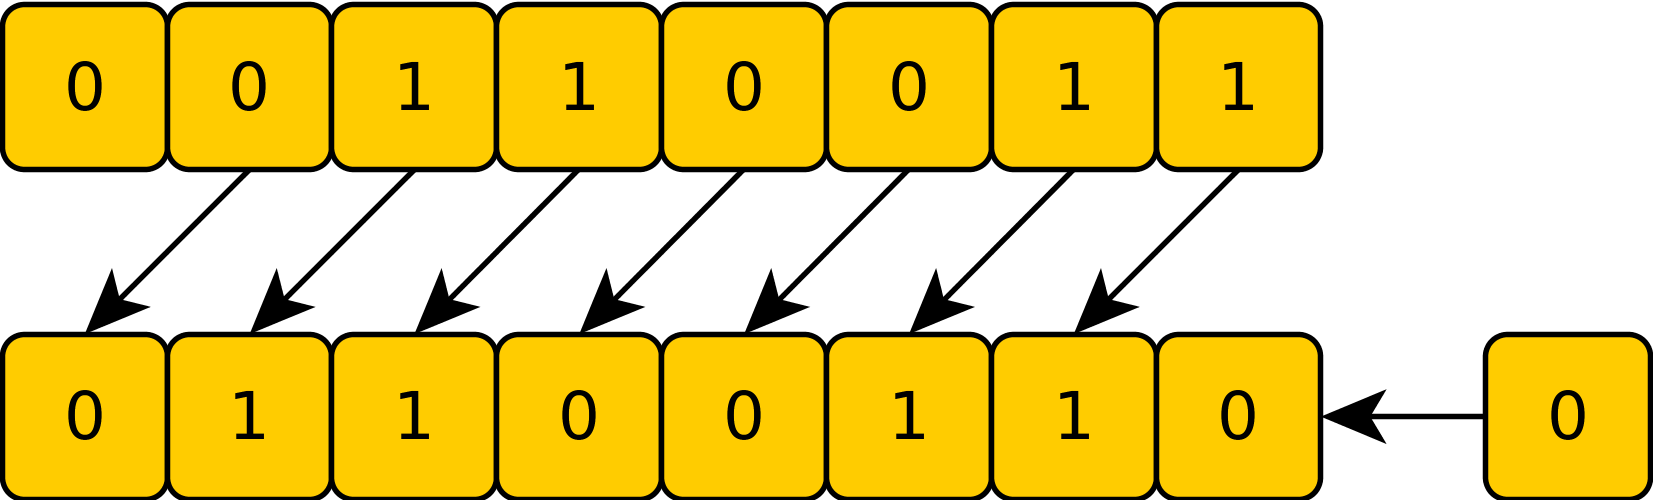
\includegraphics[height=1.4cm]{lsl.png}
        \end{center}
        \lstinputlisting{03_bw_lsh_trap.c}
    }
    \only<2>{
        \begin{itemize}
            \item Right shift \texttt{\rsh}
        \end{itemize}
        \begin{tabular}{cc}
            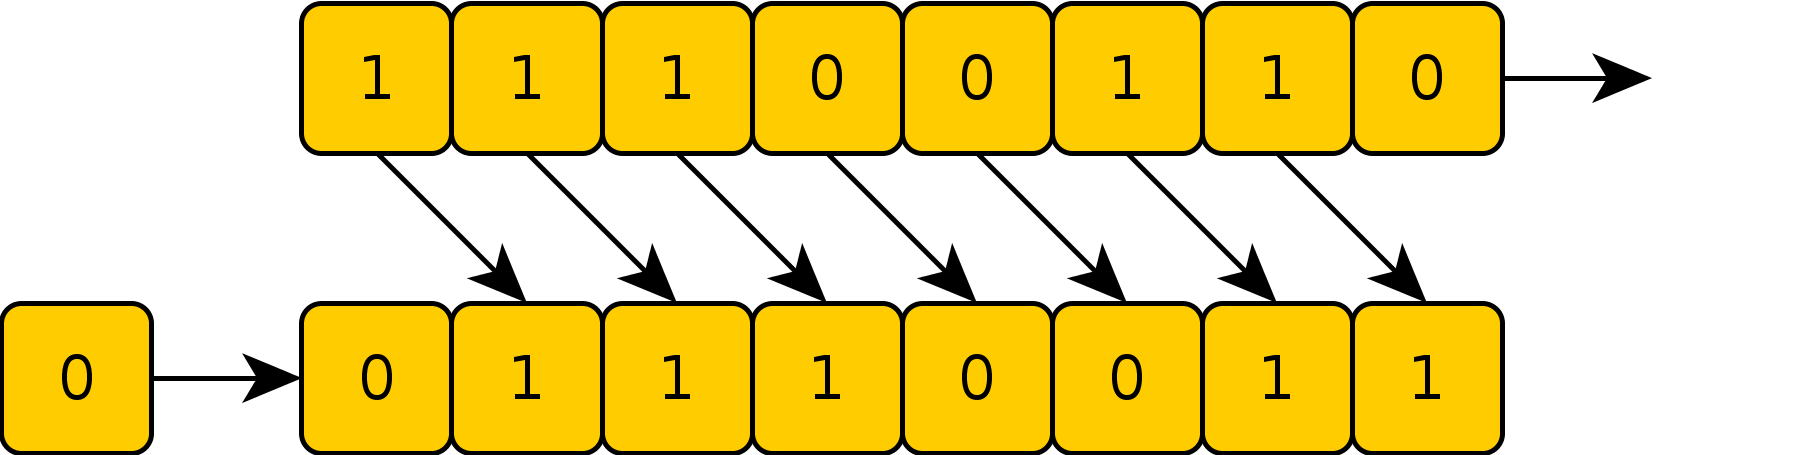
\includegraphics[height=1.4cm]{lsr.png} & 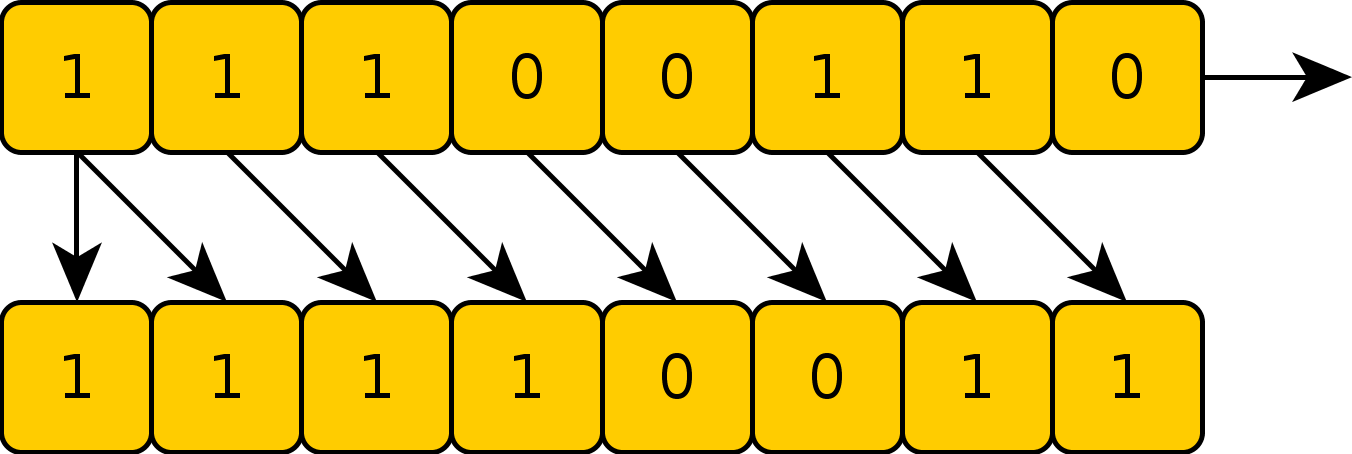
\includegraphics[height=1.4cm]{asr.png}
        \end{tabular}
        \lstinputlisting{03_bw_rsh_trap.c}
    }
\end{frame}
%%%%%%%%%%%%%%%%%%%%%%%%%%%%%%%%%%%%%%%%%%%%%%%%%%%%%%%%%%%%%%%%%%%%%%%%%%%%%%%
\begin{frame}{Short-circuiting behaviour of \texttt{\&\&} and \texttt{||}}
    \lstinputlisting{03_short_circuit.c}
\end{frame}
%%%%%%%%%%%%%%%%%%%%%%%%%%%%%%%%%%%%%%%%%%%%%%%%%%%%%%%%%%%%%%%%%%%%%%%%%%%%%%%
\begin{frame}{Maximum Munch rule}
    \only<1>{
        \lstinputlisting{03_max_munch_01.c}
    }
    \only<2>{
        \begin{block}{C11 \textsection{6.4.4} Lexical elements}
            \justifying
            If the input stream has been parsed into preprocessing tokens up to a given character,
            the next preprocessing token is the longest sequence of characters that
            could constitute a preprocessing token.
        \end{block}
        \begin{block}{}
            \justifying
            In other words the tokenizer should keep reading characters from the source file until adding
            one more character causes the current token to stop making sense. If there's more than one
            possibility for the next token, the tokenizer will prefer to bite off the one involving
            the longest sequence of characters.
        \end{block}
    }
    \only<3>{
        \lstinputlisting{03_max_munch_02.c}
    }
    \only<4>{
        \lstinputlisting[language=]{03_max_munch_03.c}
    }
    \only<5>{
        \lstinputlisting[language=c++]{03_max_munch_cpp.cpp}
    }
    \only<6>{
        \lstinputlisting[language=c]{03_max_munch_04.c}
    }
\end{frame}
%%%%%%%%%%%%%%%%%%%%%%%%%%%%%%%%%%%%%%%%%%%%%%%%%%%%%%%%%%%%%%%%%%%%%%%%%%%%%%%
\begin{frame}{Sequence points}
    %
    \only<1>{
        \lstinputlisting{03_sequence_points.c}
    }
    \only<2>{
            \justifying
            A \textbf{sequence point} defines any point in a computer program's
            execution at which it is guaranteed that all side effects of previous
            evaluations will have been performed, and no side effects from
            subsequent evaluations have yet been performed. \\
        \begin{itemize}
            \justifying
            \item Between evaluation of the left and right operands of
                  the \texttt{\&\&}, \texttt{||} and comma operators.
            \item Between evaluation of the first operand of the ternary
                  "question-mark" operator and the second or third operand.
            \item At the end of a full expression (assignment, \kwblue{return} statement,
                  \kwblue{if}, \kwblue{switch}, \kwblue{while}, \kwblue{do-while}
                  statements, all three expressions in a \kwblue{for} statement),
                  at the end of an initializer.
            \item Before a function is entered in a function call.
        \end{itemize}
    }
    \only<3>{
        \lstinputlisting{03_sp_f.c}
    }
\end{frame}
%%%%%%%%%%%%%%%%%%%%%%%%%%%%%%%%%%%%%%%%%%%%%%%%%%%%%%%%%%%%%%%%%%%%%%%%%%%%%%%
\begin{frame}{Integer promotion}
    \note{Explain what is side-effect}
    \only<1>{
        \begin{block}{Integer promotion}
        \justifying
        Integer types smaller than int are promoted when an operation is
        performed on them. If all values of the original type can be
        represented as an int, the value of the smaller type is converted to
        an int; otherwise, it is converted to an unsigned int. Integer
        promotions are applied as part of the usual arithmetic conversions
        to certain argument expressions; operands of the unary \texttt{+},
        \texttt{-}, and \textasciitilde{} operators; and operands of
        the shift operators.
        \end{block}
    }

    \only<2>{
        \lstinputlisting{03_bitwise_int_prom_trap.c}
    }
\end{frame}
%%%%%%%%%%%%%%%%%%%%%%%%%%%%%%%%%%%%%%%%%%%%%%%%%%%%%%%%%%%%%%%%%%%%%%%%%%%%%%%
\begin{frame}{Summary}
    \begin{itemize}
        \item Use parentheses when not sure about precedence rules.
        \item Be carefull with shifts (especially when shifting signed types).
        \item Understand sequence points.
        \item Understand integer promotion rules.
    \end{itemize}
\end{frame}
%%%%%%%%%%%%%%%%%%%%%%%%%%%%%%%%%%%%%%%%%%%%%%%%%%%%%%%%%%%%%%%%%%%%%%%%%%%%%%%


%\begin{frame}{Arithmetic conversion}
%If both operands have the same type, then no further conversion is needed.
%
%Otherwise, if both operands have signed integer types or both have unsigned integer types, the operand with the type of lesser integer conversion rank is converted to the type of the operand with greater rank.
%
%Otherwise, if the operand that has unsigned integer type has rank greater or equal to the rank of the type of the other operand, then the operand with signed integer type is converted to the type of the operand with unsigned integer type.
%
%Otherwise, if the type of the operand with signed integer type can represent all of the values of the type of the operand with unsigned integer type, then the operand with unsigned integer type is converted to the type of the operand with signed integer type.
%
%Otherwise, both operands are converted to the unsigned integer type corresponding to the type of the operand with signed integer type.
%\end{frame}


% int a  = 5000
% int b = 25
% long c = a *b
% a*b is evaluated using integer arithmetic, this code fine on machines with 32 integers, but overflow on 16 bit so c is initialized to the wrong value
% Addison Wesley - pointers on C
%

\end{document}
